% Preamble
\documentclass[11pt, a4paper]{article}
\usepackage[spanish]{babel}

% Packages
\usepackage{amsmath}
\usepackage[T1]{fontenc}
\usepackage{lmodern}
\usepackage{lipsum}
\usepackage{hyperref}
\usepackage{listings}
\usepackage{algorithm}
\usepackage{algpseudocode}
\usepackage{algorithmicx}
\usepackage{caption}
\usepackage{graphicx}
\usepackage{setspace}

% Redefine caption label format
\captionsetup[algorithm]{labelsep=colon, name=Algoritmo}

% Document
\begin{document}

    \begin{titlepage}
        \begin{center}
            \begin{spacing}{1.5}
                \centering
                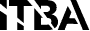
\includegraphics[width=0.2\textwidth]{./itba}
            \end{spacing}
            {\scshape\Large Instituto Tecnológico de Buenos Aires}
            {\rule{\textwidth}{0.4pt}}
            {\textbf{72.25 - Simulación de Sistemas }}
        \end{center}

        \vspace{35mm}

        \begin{center}
            \begin{spacing}{1.5}
                {\LARGE{\textbf{AUTÓMATAS CELULARES: BANDADAS DE AGENTES AUTOPROPULSADOS}}}
            \end{spacing}
        \end{center}

        \vspace{50mm}

        \begin{minipage}[t]{0.47\textwidth}
            \begin{center}
                {\textbf{Alejo Flores Lucey}}
                \\
                Legajo 62622
                \\
                {afloreslucey@itba.edu.ar}
            \end{center}
        \end{minipage}
        \hfill
        \begin{minipage}[t]{0.47\textwidth}
            \begin{center}
                {\textbf{Nehuén Gabriel Llanos}}
                \\
                Legajo 62511
                \\
                {nllanos@itba.edu.ar}
            \end{center}
        \end{minipage}

        \vspace{25mm}

        \begin{center}
            {\large{\textbf{2024 1C}}}
            \\
            {\large{Grupo Nº3}}
        \end{center}
    \end{titlepage}

    \section{Introducción}

        En este trabajo práctico se presentará el análisis de la implementación computacional del modelo Off Latice, que busca
        representar el comportamiento de un sistema de partículas autopropulsadas en un espacio bidimensional. El estudio que se
        realiza a continuación se basa en el paper \textit{Novel Type of Phase Transition in a System of Self-Driven Particles} de
        \textit{Tamás Vicsek, András Czirók, Eshel Ben-jacob, Inon Cohen y Ofer Shochet}, publicado en 1995.

        La implementación del modelo permite simular el sistema de partículas y definir observables que permiten estudiar el
        comportamiento del mismo en función de la variación de los parámetros de entrada. En este sentido, se estudiarán los
        observables Parámetro de Orden, Visitas Periodic Boundary Conditions (PBC) y Visitas Open Boundary Conditions (OBC).

        \subsection{Sistema Real}


            El modelo Off Latice busca analizar el movimiento de un conjunto de partículas cuando estas interactúan entre sí y
            como se produce un efecto de agrupamiento entre ellas a medida que el tiempo transcurre. Este fenómeno se lo conoce
            como movimiento colectivo en la naturaleza y es observado en comportamientos como el vuelo de bandadas de pájaros,
            el desplazamiento de cardúmenes de peces, entre otros. Además, se manifiesta a nivel microscópico en sistemas como
            el movimiento de bacterias y las células.

        \subsection{Fundamentos}

            El modelo de Bandadas de Agentes Autopropulsados se basa en dos ecuaciones principales. La primera de ellas:
            \begin{equation}
                x_i(t+1) = x_i(t) + v_i(t) \Delta t
            \end{equation}
            Donde $x_i(t)$ es la posición de la partícula i-ésima en el instante de tiempo $t$, $v_i(t)$ es la velocidad de la partícula i-ésima
            y $\Delta t$ es el paso de tiempo.
            Por otro lado, tenemos la segunda ecuación:
            \begin{equation}
                \theta(t+1) = \langle \theta(t) \rangle_r+ \Delta \theta
            \end{equation}
            Donde $\langle \theta(t) \rangle_r$ es el promedio de los ángulos de todas las partículas dentro de $r$ incluyendo la propia
            partícula:
            \begin{equation}
                \langle \theta(t) \rangle_r = atan2(\langle sin(\theta(t)) \rangle_r, \langle cos(\theta(t)) \rangle_r)
            \end{equation}
            y $\Delta \theta$ es el ruido uniforme entre $[-\eta/2, \eta/2]$.

    \newpage

    \section{Implementación}

    La implementación del modelo matemático de autómatas autopropulsados se realizó en dos lenguajes de programación:
    \begin{itemize}
        \item Java: en su versión 19 en conjunto con Maven para la gestión de dependencias.
        \item Python: en su versión 3.8.5 con las librerías numpy, matplotlib y pandas.
    \end{itemize}

    Java se utilizó para la implementación del modelo Off Latice, mientras que Python se utilizó para la creación de las
    animaciones y la obtención de los gráficos que muestran los resultados de los observables estudiados.

    Para iniciar el desarrollo de este modelo computacional, se partió del código realizado en el Trabajo Práctico Nro. 1 que
    implementaba el Cell Index Method en Java. Este método permite obtener las partículas vecinas de una partícula en específico
    considerando un radio y un conjunto de celdas determinado. Esta implementación posibilita la obtención del ángulo que tendrá
    la partícula a analizar en específico luego de verse afectada por los ángulos de aquellas que se consideran vecinas.

    En el proyecto Java se tienen tres clases principales. La primera de ellas es \texttt{MovingParticle}, que extiende de
    la clase \texttt{Particle} y que representa a una partícula que se mueve en el espacio. Particle es una clase utilizada en el
    TP1 y que tiene como atributos el radio de la partícula, su posición en el eje $x$, su posición en el eje $y$ y un
    identificador. \texttt{MovingParticle} hereda todos los atributos mencionados previamente y cuenta con otros dos más que son
    el ángulo de la partícula y su velocidad en un instante de tiempo.

    La segunda clase principal es \texttt{OffLatticeAutomata}, que representa el modelo de autómatas autopropulsados. La misma cuenta
    con dos atributos: el ruido que tiene el sistema y una instancia de la clase \texttt{CellIndexMethod} del TP1. El método principal de esta clase
    es el \texttt{execute()} que se encarga de crear los archivos de salida que contienen la información de las partículas del sistema
    en cada instante de tiempo teniendo en cuenta los parámetros de entrada del modelo: $N$ (cantidad de partículas), $L$ (longitud
    del lado del espacio bidimensional), $r_c$ (radio de corte), $v$ (módulo de la velocidad de las partículas), $\eta$ (ruido) y
    $t$ (la cantidad de frames o tiempos que se quieren simular).

    Por último, la tercera clase principal es \texttt{Main}. Esta se encarga de leer los parámetros de entrada de un archivo input y
    realizar la ejecución del modelo de autómatas autopropulsados. Con la información de las partículas obtenidas en los archivos
    output que se generan en este programa, se pueden llevar a cabo las animaciones y los gráficos de los observables estudiados.

        \subsection{Arquitectura}

            \begin{figure}[htbp]
                \centering
                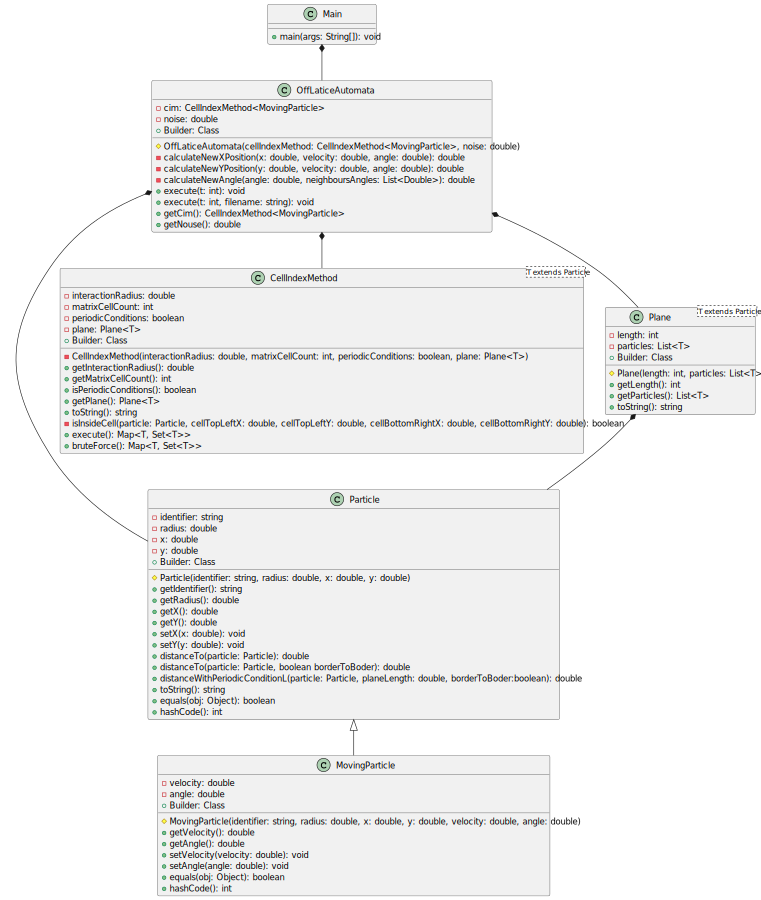
\includegraphics[height=0.69\textheight]{./Architecture}
                \caption{Arquitectura del código implementado.}
                \label{fig:my_png}
            \end{figure}

        \subsection{Algoritmo}

            La simulación del modelo de autómatas autopropulsados se basa en las dos funciones principales descritas en la sección
            de Fundamentos y a continuación se presenta el modelo computacional en pseudo-código que se ha implementado:

            \begin{algorithm}
                \caption{Off Latice Automata}
                \begin{algorithmic}[1]
                    \State Se crea una archivo de salida para el instante de tiempo $t$
                        \While{$t < t_{max}$}
                            \State Ejecución de CellIndexMethod
                            \State Obtención de las partículas vecinas de cada partícula en $t$
                            \State Creación de una lista de objetos Partícula - ÁngulosVecinas en $t$
                            \While{Partícula en List de Partículas - ÁngulosVecinas}
                                \State Cálculo del ángulo promedio de las partículas vecinas
                                \State Definición del nuevo ángulo de la partícula en $t+1$
                                \State Actualización de la posición en $x$ de la partícula en $t+1$
                                \State Actualización de la posición en $y$ de la partícula en $t+1$
                                \State Incremento del instante de tiempo $t$
                                \State Escritura de la información de la partícula en archivo output
                            \EndWhile
                        \EndWhile
                \end{algorithmic}
            \end{algorithm}

            Una observación importante a tener en cuenta es que el \texttt{CellIndexMethod} retorna un mapa, es decir, una estructura
            que está conformada por una clave y un valor. En este caso, la clave es una partícula y el valor es una lista con todas
            las partículas vecinas de la misma.
            Otro aspecto relevante a mencionar es que la lista formada por objetos del tipo Partícula - ÁngulosVecinas
            tiene copias y no referencias de los ángulos correspondientes a las partículas vecinas. Esto es así para evitar que la actualización de un
            ángulo no se vea afectada por la actualización de otro ángulo en el mismo instante de tiempo.

    \newpage

    \section{Simulaciones}

        En esta sección se describirá el sistema particular que se va a simular y estudiar. Para ello, se
        presentarán aspectos como la geometría, el rango de parámetros fijos y variables, los inputs y outputs
        y se definirán los observables que se calcularán a partir del output de la simulación.

        Se ha decidido mantener fijos los siguientes parámetros en todas las simulaciones:
        \begin{itemize}
            \item $r_c = 1$
            \item $v = 0,03$
            \item $L = 5$
        \end{itemize}
        Donde los primeros dos tienen los mismos valores que los presentes en el paper de referencia
        compartido por la cátedra y el último se ha decidido mantener constante para poder realizar comparaciones
        y observaciones más claras.

        Las simulaciones realizadas buscan obtener resultados sobre como determinados observables escalares varían
        en función de los parámetros variables. Aquellos obserables a analizar son:
        \begin{itemize}
            \item Parámetro de Orden: $v_a$.
            \item Visitas Periodic Boundary Conditions (PBC): tiempo en el que el nro. de visitas alcanza un dado porcentaje de N.
            \item Visitas Open Boundary Conditions (OBC): nro. de visitas por unidad de tiempo.
        \end{itemize}
        Los parámetros variables son:
        \begin{itemize}
            \item $N$: Cantidad de partículas.
            \item $\eta$: Ruido.
        \end{itemize}

        A continuación se describirá el sistema particular elegido para cada observable escalar a estudiar.

        \subsection{Parámetro de Orden ($v_a$)}
            Este primer observable escalar se define como:
            \begin{equation}
                v_a = \frac{1}{Nv} \left|\sum_{i=1}^{N} \vec{v_i} \right|
            \end{equation}
            Donde N representa la cantidad de partículas y $v$ es el módulo de la velocidad de las mismas. Por último,
            se tiene al valor absoluto de la sumatoria de todos los vectores $\vec{v_i} \  \backslash \  0 \geq i \leq N$,
            que representan el vector velocidad de la partícula i-ésima. El valor del Parámetro de Orden tiende a cero
            (0) cuando las partículas se encuentran en total desorden, por otro lado, tiende a uno (1) cuando las partículas
            se encuentran polarizadas.

        \subsection{Visitas PBC: tiempo en el que el nro. de visitas alcanza un dado porcentaje de N.}
            En este caso, la simulación consta de un sistema de partículas que se mueven en una celda de lado $L$,
            pero con la particularidad de que se tienen cuatro (4) zonas de conteo circulares fijas de radio $0,5$ y la
            ubicación de las mismas es igual para todas las simulaciones y todos los $\eta$.

            Al ser un Periodic Boundary Conditions, se consideran los id's de las partículas que ingresan a la zona de
            conteo y por lo tanto, cada partícula solo debe ser contabilizada una vez al visitar cada zona de medición.
            El observable a estudiar es el tiempo en el que el número de visitas alcanza el 20\% de N dependiendo
            del $\eta$ (ruido).

            Esta simulación se realiza para cuatro (4) N's distintos ($100$, $300$, $500$ y $1000$) y para cada uno de ellos
            se varía el $\eta$ en un rango de $0$ a aproximadamente $5,8$ con un paso de $0,2$. Es interesante analizar la
            obtención de los resultados de las simulaciones puesto que se tienen cuatro (4) zonas circulares fijas ubicadas en lugares
            distintos. En consecuencia, para poder el obtener el valor del observable, primero se deben promediar los tiempos obtenidos
            de cada una de las zonas de conteo de la siguiente manera:
            \begin{equation}
                t_{\text{prom}} = \frac{1}{4} \sum_{i=1}^{4} t_i \ ,\ t_i\text{: tiempo en la zona }i
            \end{equation}
            Al ser un promedio entre cuatro (4) valores, es necesario calcular el error mediante desvío estándar:
            \begin{equation}
                \sigma = \sqrt{\frac{1}{4} \sum_{i=1}^{4} (t_i - t_{\text{prom}})^2}
            \end{equation}
            Con estos dos valores obtenidos se obtendrá el valor del observable y su error en función del $\eta$ para cada N de los mencionados previamente.


    \subsection{Visitas OBC: nro. de visitas por unidad de tiempo.}
            El sistema que se simula en este caso es el mismo que se describe en el primer apartado de la subsección
            anterior, pero con la particularidad de que ahora es un Open Boundary Conditions. Esta condición refiere
            al hecho de que no se considerarán los id's de las partículas a la hora de ingresar a las zonas de conteo,
            por lo que una misma partícula reingresa a la zona de medición será contabilizada nuevamente.

            El observable a estudiar es el número de visitas por unidad de tiempo dependiendo del $\eta$ (ruido), es decir,
            la pendiente de la curva número de visitas vs tiempo en la zona donde esta sea estacionaria.
            Esta simulación, al igual que la descrita en el apartado anterior, se realiza para los mismos cuatro (4) N's
            ($100$, $300$, $500$ y $1000$) y también se varía el $\eta$ en el mismo rango (de $0$ a aproximadamente $5,8$)
            con un paso de $0,2$.

            Como el objetivo es obtener la pendiente de la curva número de visitas vs tiempo, es necesario obtener las curvas
            de cada una de las cuatro (4) zonas de conteo. Dado que el caracter de estas curvas es no lineal, es imperioso
            obtener la pendiente de la recta asociada a cada una de ellas mediante el método de regresión lineal simple, que
            es un método que permite aproximar la relación de dependencia entre una variable independiente $y$ (cantidad de visitas)
            y un conjunto de variables independientes $x$ (tiempo). La definición de la recta asociada es la siguiente:
            \begin{equation}
                y = \beta_0 x + \beta_1
            \end{equation}

            Como se puede observar, existen dos coeficientes $\beta_0$ y $\beta_1$ que no se conocen. Como para el estudio que se
            está realizando solamente es de interés la pendiente, se puede obviar el cálculo de $\beta_1$ y obtener directamente
            el valor de $\beta_0$ con la siguiente fórmula:
            \begin{equation}
                \beta_0 = \frac{\sum_{i=1}^N x_i y_i - N\bar{x} \bar{y}}{\sum_{i=1}^N x_i^2 - \frac{1}{N} \left(\sum_{i=1}^N x_i \right)^2}
            \end{equation}

            Este coeficiente representa el valor de la pendiente de la recta asociada a la curva de visitas en función de tiempo y
            debido a que es una pendiente, de ahora en más se la llamará $m$:
            \begin{equation}
                m_k = \frac{\sum_{i=1}^N x_i y_i - N\bar{x} \bar{y}}{\sum_{i=1}^N x_i^2 - \frac{1}{N} \left(\sum_{i=1}^N x_i \right)^2}
                \ , 1 \leq k \leq 4
            \end{equation}
            En el numerador se tiene a la diferencia entre la sumatoria de los productos de las variables independientes y dependientes
            y el producto entre $N$ y las medias de las variables independientes y dependientes.
            Por otro lado, en el denominador se tiene a la diferencia entre la sumatoria de los cuadrados de las variables independientes
            y el producto entre el inverso de $N$ y la sumatoria de las variables independientes al cuadrado. El $k$ representa la zona
            de conteo a la que se le está calculando la pendiente.

            Para poder obtener un valor único del observable, es necesario obtener el promedio de las pendientes de las cuatro (4) zonas:
            \begin{equation}
                m_{prom}(N,\eta) = \frac{1}{4} \sum_{i=1}^{4} m_i \ , 1 \leq i \leq 4
            \end{equation}
            Además, por su condición de promedio debemos obtener el error asociado mediante el desvío estándar:
            \begin{equation}
                \sigma = \sqrt{\frac{1}{4} \sum_{i=1}^{4} (m_i - m_{prom})^2}
            \end{equation}
            Con estas consideraciones pobremos obtener los diferentes valores del observable en y su error en función del $\eta$
            para cada N de los mencionados previamente.

    \newpage

    \section{Resultados}

    Estructurar la sección de resultados de la siguiente manera.
    2.4.1 Para cada input o parámetro a estudiar, primero mostrar una animación característica del
    sistema (pueden ser dos, con dos valores extremos del input para ver ejemplos de distintos
    comportamientos). La idea de esto es ilustrar la dinámica del sistema para situar el contexto de los
    resultados a mostrar.
    2.4.2 Luego mostrar una figura del observable o métrica (que se calcula a partir de los outputs
    directos de la simulación) en función del tiempo. Explicar entonces cual será el escalar que
    caracteriza ese proceso (por ejemplo el promedio de la evolución temporal en el estado
    estacionario, la tasa de crecimiento, etc.). Solo mostrar evoluciones típicas, de valores extremos
    del rango de parámetros, para validar las definiciones de los observables. Las evoluciones en sí
    no son los resultados definitivos, por lo tanto no deben ser extenso lo que se muestre de las
    mismas solo para justificar el observable (escalar) que se calculará a partir de estas.
    2.4.3 Después presentar la figura del input vs. observable, con promedio y barras de error o tablas
    con promedio y error.
    2.4.4 Repetir los pasos desde 2.4.1 hasta 2.4.3 para los otros parámetros o inputs que se
    estudiaron.
    2.4.5 Cuando se ajuste una función teórica a los resultados de las simulaciones se debe mostrar
    como se halló el mejor ajuste en los términos de lo explicado en la Teórica 0.
    2.4.6 Las Figuras deben tener los datos promedios obtenidos claramente identificados con un
    símbolo (o la barra de error). No se pueden unir los puntos con lineas sin destacar cuales son los
    puntos. Estos datos pueden ser opcionalmente unidos por lineas rectas como "guía para el ojo".
    En ningún caso se puede interpolar los datos con funciones arbitrarias (polinomios, splines) que
    no provengan de ninguna teoría sobre el sistema que se estudia.
    2.4.7 Cuando los datos varían en distintos ordenes de magnitud (incluso con potencias negativas,
    por ejemplo para una función que tiene una asíntota en cero) una escala lineal puede no permitir
    que se distingan visualmente las diferencias, en esos casos se debe graficar con escala doble
    logarítmica o semilogarítmica en el eje que corresponda.
    2.4.8 Durante la presentación en vivo (presencial o virtual) las animaciones debe estar embebidas
    en la diapositiva correspondiente (no salir de la presentación para mostrarlas con otro programa).
    Pero en el archivo pdf de la presentación que se debe entregar no debe haber animacionesembebidas, ni tampoco se deben entregar archivos de animaciones. La presentación en formato
    pdf debe tener una imagen fija de un fotograma representativo de la animación y debajo de este
    debe estar explícitamente escrito un link a youtube o similar.


    \section{Conclusiones}

        Basadas solo en los resultados mostrados, no son conclusiones
        resultados observados pero no mostrados en resultados, ni hipótesis de posibles explicaciones de
        lo observado que no hayan sido estudiadas explícitamente, cualquier hipótesis que
        potencialmente explique lo observado, debe ser probada explícitamente y mostrada en resultados,
        caso contrario no es válida como conclusión. Tampoco es una conclusión algo que haya quedado
        por hacer o algo que se haya hecho mal y se descartó.
        2.6 Puede haber una diapositiva de cierre con algún tipo de agradecimiento", pero no se estila en
        la misma escribir la palabra "preguntas?"


\end{document}
